\documentclass[aspectratio=149]{beamer}
\usepackage[english]{babel}
\usepackage{uep_kie_ms}
\usepackage{makecell}

\setbeamertemplate{footline}[text line]{
\includegraphics[height=0.7cm]{logo_uep}
\hspace*{8cm}~%

\includegraphics[height=0.7cm]{logo_ncbr_en}
}

\author{Marcin~Sawiński \and 
Krzysztof~Węcel \and 
Ewelina~Księżniak \and 
Milena~Stróżyna \and 
Włodzimierz~Lewoniewski \and
Piotr~Stolarski \and
Witold~Abramowicz}
\date{2023-09-21}
\institute{Poznań University of Economics and Business} 
\title{OpenFact at CheckThat! 2023: Head-to-Head GPT vs. BERT - A Comparative Study of Transformers Language Models for the Detection of Check-worthy Claims}
\subtitle{Notebook for the CheckThat! Lab at CLEF 2023}

\begin{document}

\begin{frame}
\begin{figure}
\includegraphics[height=1cm]{logo_clef}
\hspace*{0.5cm}~%
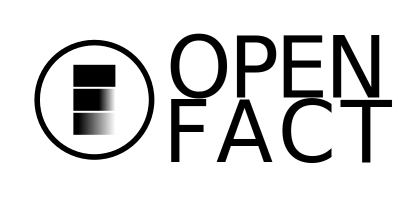
\includegraphics[height=1cm]{logo_openfact}
\hspace*{0.5cm}~%

\includegraphics[height=1cm]{logo_infos.png}
\hspace*{0.5cm}~%

\includegraphics[height=1cm]{logo_godlo_flaga}
\end{figure}
\fontsize{7pt}{7pt}\selectfont
OpenFact -- AI tools for verification of veracity of information sources and fake news detection.\\ Financed by National Center for Research and Development in Poland (INFOSTRATEG-I/0035/2021-00).

\titlepage
\end{frame}
%%%%%%%%%%%%%%%%%%%%%%%%%FRAME%%%%%%%%%%%%%%%%%%%%%%%%%
\begin{frame}{Experiments}
\begin{itemize}
  \item Tasks: \emph{Check-That! Lab, Task 1B-English} 
  \item Dataset: ClaimBuster (23,533 statements extracted from all U.S. general election presidential debates). Splits:\begin{itemize}
  \item train \& dev - ClaimBuster crowd-sourced 
  \item dev\_test - ClaimBuster ground-truth
\end{itemize}

  \item Methods:\begin{itemize}
  \item GPT
  \item BERT
  \item Ensemble
\end{itemize}
\end{itemize}
\end{frame}
%%%%%%%%%%%%%%%%%%%%%%%%%FRAME%%%%%%%%%%%%%%%%%%%%%%%%%
\begin{frame}{Curating dataset - volume vs quality vs usefulness}
\begin{itemize}

  

  \item 'Dataset Cartography: Mapping and Diagnosing Datasets with Training Dynamics' - Swayamdipta 2020
    \item 'Scaling Laws for Neural Language Models' - Kaplan 2020
    \item 'Textbooks Are All You Need' - Gunasekar 2023
\end{itemize}

%\begin{figure}[h]
%    \centering
%    \includegraphics[width=10cm]{../fig/kaplan}
%\caption{A series of language model training runs, with models ranging in size from $10^3$ to $10^9$ parameters (excluding embeddings). Source: Scaling Laws for Neural Language Models (kaplan 2020)}
%    \label{fig:kaplan}
%\end{figure}
\end{frame}

%%%%%%%%%%%%%%%%%%%%%%%%%FRAME%%%%%%%%%%%%%%%%%%%%%%%%%
\begin{frame}{Curating dataset - fewer, better data}
\begin{itemize}
  \item Original train data set size - 16821
  \item Curated train data set size 2:1 NCS/CS - 7692

\end{itemize}

\begin{figure}[h]
    \centering
    \includegraphics[width=10cm]{./sank}
\caption{Reshuffling of 2:1 dataset}
\end{figure}
\end{frame}

%%%%%%%%%%%%%%%%%%%%%%%%%FRAME%%%%%%%%%%%%%%%%%%%%%%%%%
\begin{frame}{GPT in-context learning}
\begin{itemize}
  \item Zero-shot learning using GPT-4
  \begin{itemize}
  \item System prompt
  \item Explanation of task
  \item Multiple phrasing variants
  \item Mini-batches
\end{itemize}
  \item Few-shot learning using GPT-4
\begin{itemize}
  \item System prompt 
  \item Aassistant prompts
  \item 4 yes and 4 no examples based on cosine similarity of  all-mpnet-base embeddings
\end{itemize}
  \item Few-shot learning with Chain-of-Thought using GPT-4
  \begin{itemize}
  \item  multi-step assistant prompts (claim, opinion,topic, topic type, harmful)
\end{itemize}

\end{itemize}
\end{frame}
%%%%%%%%%%%%%%%%%%%%%%%%%FRAME%%%%%%%%%%%%%%%%%%%%%%%%%
\begin{frame}{Fine-tuning OpenAI GPT-3}
\begin{itemize}
  \item The Curie model - 13 billion parameters, trained using 800GB of text data.
  \item The Davinci model - 175 billion parameters  trained using 45TB of text data3.
  \item Using only 50\% of training data
\end{itemize}

\begin{table}[h]
\centering

\label{tab:finetuning-hyperparams}
\begin{tabular}{lc}
        \toprule
        \textbf{Hyperparameter}        & \textbf{Value} \\
        \midrule
        Batch size                     & 8              \\ 
        Learning rate multiplier       & 0.1            \\ 
        Epochs                         & 4              \\ 
        Prompt loss weight             & 0.01           \\ 
        Compute classification metrics & True           \\ 
\bottomrule
    \end{tabular}
\caption{Hyperparameters used for fine-tuning GPT-3 models}
\end{table}
\end{frame}
%%%%%%%%%%%%%%%%%%%%%%%%%FRAME%%%%%%%%%%%%%%%%%%%%%%%%%
\begin{frame}{BERT - Model Fine-tuning and Technical Constraints}
    % \frametitle{Model Fine-tuning and Technical Constraints}
    \begin{itemize}
        \item Models fine-tuned: DistilBERT, DeBERTa, RoBERTa, XLM-RoBERTa, ALBERT, RemBERT, CamemBERT, ELECTRA, YOSO
        \item Technical constraints:  Local machine setup - four NVIDIA GeForce RTX 2080 Ti GPU cards, 11 GB of memory per card
        \item Techniques to reduce memory usage: batch size adjustments: 16 to 8 or 4, gradient accumulation float precision: FP16 and FP32
        
        \end{itemize}
\end{frame}



\begin{frame}{BERT - Hyperparameterization}
    % \frametitle{Hyperparameterization}
    \begin{itemize}
        \item Optimizer: AdamW, Adafactor for RemBERT model
        \item Learning rates: 2e-5 (default), 1e-5, 3e-5
        \item Fine-tuning duration: 5 epochs (20-30 minutes), extended to 10 epochs if necessary
        \item Fine-tuning with Layer-wise LR Decay
        \item Training objective: F1 macro average, F1 positive optimized
    \end{itemize}
    
\end{frame}





\begin{frame}
% \todo{moze tabelka z przykladowymi featurami}
    \frametitle{Light GBM – Ensemble Approach}
    \begin{itemize}
        \item Approach: Combine predictions from fine-tuned models
        \begin{itemize}
            \item Predicted labels and probabilities
            \item Emotion and sentiment probabilities from models BERTemo model
            \item Logits returned by ELECTRA discriminator (logit of the first token, the logit of the last token, the minimum logit value, the mean logit value, the maximum logit value, the number of odd tokens (when logit is bigger than zero), and the percentage of odd tokens)
        \end{itemize}
        \item Best F1 score: 0.79 (despite various hyperparameter settings)
        \item The most important feature: probabilities from fine-tuned DeBERT-a
    \end{itemize}
\end{frame}

%%%%%%%%%%%%%%%%%%%%%%%%%FRAME%%%%%%%%%%%%%%%%%%%%%%%%%
\begin{frame}{Experiments results}
\fontsize{9pt}{10pt}\selectfont
\begin{table}[!htb]
    \centering
%    \caption{The results obtained by the GPT and BERT models}
    \label{tab:results}
    \begin{tabular}{lrrrr}
        \toprule
        Model                              & F1    & precision & recall & accuracy \\
        \midrule
        GPT-3 curie fine-tuned curated     & 0.898 & 0.948     & 0.852  & 0.934    \\
        DeBERTa v3 base fine-tuned         & 0.894 & 0.978     & 0.824  & 0.934    \\
        GPT-3 davinci fine-tuned curated   & 0.876 & 0.946     & 0.815  & 0.921    \\
        RoBERTa base fine-tuned            & 0.862 & 0.966     & 0.778  & 0.915    \\
        \makecell[l]{RoBERTa base fine-tuned with custom                           \\optimizer layer-wise learning rate decay} & 0.860 &      0.976 &   0.769 &     0.915 \\
        \makecell[l]{LightGBM ensemble of all BERT-based                           \\models and additional embeddings} & 0.854 &      0.976 &   0.759 &     0.912 \\
        ELECTRA fine-tuned                 & 0.851 & 0.954     & 0.769  & 0.909    \\
        AlBERT large v2 fine-tuned         & 0.848 & 0.976     & 0.750  & 0.909    \\
        DistilBERT base uncased fine-tuned & 0.827 & 0.952     & 0.731  & 0.896    \\
        GPT-3 curie fine-tuned random      & 0.826 & 1.000     & 0.704  & 0.899    \\
        GPT neo 125M fine-tuned            & 0.800 & 0.961     & 0.685  & 0.884    \\
        GPT-4 few-shot learning            & 0.788 & 0.867     & 0.722  & 0.868    \\
        GPT-4 zero-shot learning           & 0.778 & 0.710     & 0.861  & 0.833    \\
        GPT-4 Chain-of-Thought             & 0.722 & 0.574     & 0.972  & 0.745    \\
        \bottomrule
    \end{tabular}

\end{table}
\end{frame}
%%%%%%%%%%%%%%%%%%%%%%%%%FRAME%%%%%%%%%%%%%%%%%%%%%%%%%
\begin{frame}{Experiments results on curated dataset}
\fontsize{9pt}{10pt}\selectfont
\begin{table}[!htb]
    \centering
%    \caption{The results obtained by the GPT and BERT models}
    \label{tab:results}
\begin{tabular}{lrrrr}
\toprule
                        Model &    f1 &  precision &  recall &  accuracy \\
\midrule
  GPT-3 curie fine-tuned curated & 0.898 &      0.948 &   0.852 &     0.934 \\
            RoBERTa base curated & 0.896 &      0.968 &   0.833 &     0.934 \\
      DeBERTa v3 base fine-tuned & 0.894 &      0.978 &   0.824 &     0.934 \\
GPT-3 davinci fine-tuned curated & 0.876 &      0.946 &   0.815 &     0.921 \\
         RoBERTa base fine-tuned & 0.862 &      0.966 &   0.778 &     0.915 \\
   GPT-3 curie fine-tuned random & 0.826 &      1.000 &   0.704 &     0.899 \\
         DeBERTa v3 base curated & 0.818 &      0.900 &   0.750 &     0.887 \\
\bottomrule
\end{tabular}
\end{table}

\end{frame}

%%%%%%%%%%%%%%%%%%%%%%%%%FRAME%%%%%%%%%%%%%%%%%%%%%%%%%
\begin{frame}{Perspectives for future work}
			\begin{columns}
			\column{0.4\textwidth}
			\begin{itemize}
  \item More resources / bigger models / smaller models
  \item Examine dataset curation impact
  \item Chain-of-Thought and beyond
\end{itemize}
			\column{0.6\textwidth}
			\begin{figure}[h]
    \centering
    \includegraphics[width=6cm]{./f1}
\caption{Further exploration of impact of dataset/annotation quality }
\end{figure}
			\end{columns}


\end{frame}

\end{document}


